
%%%%%%%%%%%%%%%%%%%%%%%%%%%%%%%%%%%%%%%%%%%%%%%%%%%%%%%%%%%%%%%%%%%%%%%%%
%%                       Politecnico di Torino                         %%
%%   Corso  di Laurea Magistrale in Architettura Costruzione e Città   %%
%%%%%%%%%%%%%%%%%%%%%%%%%%%%%%%%%%%%%%%%%%%%%%%%%%%%%%%%%%%%%%%%%%%%%%%%%

\documentclass[11pt,a4paper]{article}
\usepackage[utf8]{inputenc}
\usepackage[italian, english]{babel}
\usepackage{geometry}
\usepackage{indentfirst} % First line indent
\usepackage{mathtools}
\usepackage{wrapfig}
\usepackage[usenames, dvipsnames]{color}
\usepackage{float}
\usepackage{amssymb}
\usepackage{ifsym}
\usepackage{abstract}
\usepackage{emptypage}
\usepackage{multicol}

\addtolength{\skip\footins}{1cm} %%%% Distanza Testo dalle Note a  piè di  pagina %%%%

%%%%%%%%%%%%%%%%%%%%%%%%%%%%%%%%%%%%%%%%%%%%%%%%%%%%%%%%
%  TIPOLOGIA TESTO TESI  %
% Testo da Revisionare: ROSSO il comando è {\color{red} di seguito il testo da mattere in rosso.}
% Testo già Revisionato: NERO quando già revisionato eliminare il comando precedente
%%%%%%%%%%%%%%%%%%%%%%%%%%%%%%%%%%%%%%%%%%%%%%%%%%%%%%%%

% Linea sopra con numero di pagina  e scritta a sx
%%%%%%%%%%%%%%%%%%%%%%%%%%%%%%%%%%%%%%%%%%%%%%%%%%%%%%%%
\usepackage{fancyhdr}
\pagestyle{fancy}
\rhead[\fancyplain{}{\bfseries\leftmark}]{\fancyplain{}{\bfseries\thepage}}
\cfoot{}
%%%%%%%%%%%%%%%%%%%%%%%%%%%%%%%%%%%%%%%%%%%%%%%%%%%%%%%%

% Misure Documento
\geometry{ a4paper, total={170mm,257mm},left=37mm, right=35mm, top=35mm, bottom=40mm }

\newcommand{\df}{\displaystyle\frac}
\newcommand{\seq}[1]{\left<#1\right>}

\linespread{1.50} % Interlinea

%%%%%%%%%%%%%%%%%%%%%%%%%%%%%%%%%%%%%%%%%%%%%%%%%%%%%%%%
%%                   Frontespizio                     %%
%%%%%%%%%%%%%%%%%%%%%%%%%%%%%%%%%%%%%%%%%%%%%%%%%%%%%%%%
\begin{document}

\begin{titlepage}
\begin{center}
\vspace{200mm}
\vspace{15mm}
{{\huge{\textsc{Politecnico di Torino}}}}

%%%%%%%%%%%%%%%%%%%%%%%%%%%%%%%% Linee
\rule[0.1cm]{15.8cm}{0.1mm}
\rule[0.5cm]{15.8cm}{0.6mm}
%%%%%%%%%%%%%%%%%%%%%%%%%%%%%%%% Linee

\begin{center}
{\large{\textmd{Corso di Laurea Magistrale\\
in Architettura Costruzione e Città}}
\end{center}

\vspace{8mm}
\begin{center}
\vspace{3mm}
{\LARGE{\textmd{Tesi di Laurea Magistrale}}\\
\vspace{3mm}
{\Large{\textmd{Realtà Aumentata applicata all'ambiente museale}}\\
\vspace{12mm}
\end{center}

\begin{figure}[h!]
  \centering
  
\includegraphics[width=4cm]{/Users/enricopicchio/Desktop/TesiLaTex/IMG/LogoP.pdf}
\end{figure}

\vspace{12mm}
\par
\noindent
\begin{minipage}[t]{0.47\textwidth}
{\large{{\itshape{Relatore}}:\\
Massimiliano Lo Turco}}
\end{minipage}
\hfill
\begin{minipage}[t]{0.47\textwidth}\raggedleft
{\large{{\itshape{Candidato}}:\\
Enrico Picchio}}
\end{minipage}\\

\vspace{8mm}
\par
\noindent
\begin{minipage}[t]{0.47\textwidth}
{\large{{\itshape{Co-Relatrice}}:\\
Elisabetta  Caterina Giovannini}}
\end{minipage}
\hfill
\vspace{25mm}
\begin{center}
{\normalsize{\textmd{Anno Accademico 2019/2020}}
\end{center}
\end{titlepage}

%%%%%%%%%%%%%%%%%%%%%%%%%%%%%%%%%%%%%%%%%%%%%%%%%%%%%%%%
%%                    Abstract                        %%
%%%%%%%%%%%%%%%%%%%%%%%%%%%%%%%%%%%%%%%%%%%%%%%%%%%%%%%%
\newpage
\null\vspace{\stretch{1}} % Sarebbe lo spazio  soprastante
\begin{abstract}

\noindent
{\color{red} % Esempio di testo da "revisionare" in colore ROSSO
This work considers electoral competition between two office-motivated parties and an electorate with preference over policies and with a concern about candidates' personal characteristics. We analyze the role of information in elections, comparing the perfect information model to a model with imperfectly informed voters and show that ignorance of policy information leads voters to vote differently from those they would hold otherwise.}
\vspace{\stretch{2}}\null % Sarebbe lo spazio sottostante
\end{abstract}

%%%%%%%%%%%%%%%%%%%%%%%%%%%%%%%%%%%%%%%%%%%%%%%%%%%%%%%%
%%                 Ringraziamenti                     %%
%%%%%%%%%%%%%%%%%%%%%%%%%%%%%%%%%%%%%%%%%%%%%%%%%%%%%%%%
\newpage
\selectlanguage{Italian}
\null\vspace{\stretch{2}}
\\
\textnormal{Desidero esprimere la mia gratitudine al Prof. Massimiliano Lo Turco e alla Prof.ssa Elisabetta Caterina Giovannini per la guida paziente, l’incoraggiamento e i consigli che hanno fornito nel corso di questa tesi. Devo ringraziare la mia famiglia e i miei amici per avermi dato sostegno e incoraggiamento costanti durante i miei anni di studio. Questo risultato non sarebbe stato possibile senza di loro. Grazie.}
\vspace{\stretch{2}}\null

%%%%%%%%%%%%%%%%%%%%%%%%%%%%%%%%%%%%%%%%%%%%%%%%%%%%%%%%
%%                    Indice                          %%
%%%%%%%%%%%%%%%%%%%%%%%%%%%%%%%%%%%%%%%%%%%%%%%%%%%%%%%%
\newpage
\begin{flushleft}
\tableofcontents
\end{flushleft}

%%%%%%%%%%%%%%%%%%%%%%%%%%%%%%%%%%%%%%%%%%%%%%%%%%%%%%%%
%%                Lista delle Figure                  %%
%%%%%%%%%%%%%%%%%%%%%%%%%%%%%%%%%%%%%%%%%%%%%%%%%%%%%%%%
\newpage
\listoffigures

%%%%%%%%%%%%%%%%%%%%%%%%%%%%%%%%%%%%%%%%%%%%%%%%%%%%%%%%%%%%%%%%%%%%%%%%%%%%%%%%%%%%%%%%%%%%%%%%%%%%%%%%%%
%%                                               INIZIO TESI                                            %%
%%%%%%%%%%%%%%%%%%%%%%%%%%%%%%%%%%%%%%%%%%%%%%%%%%%%%%%%%%%%%%%%%%%%%%%%%%%%%%%%%%%%%%%%%%%%%%%%%%%%%%%%%%

\newpage
%%%%%%%%%%%%%%%%%%%%%%%%%%%%%%%%%%%%%%%%%%%%%%%%%%%%%%%%
\section{Introduzione}
%%%%%%%%%%%%%%%%%%%%%%%%%%%%%%%%%%%%%%%%%%%%%%%%%%%%%%%%
Lorem ipsum dolor sit amet, consectetur adipisicing elit, sed do eiusmod tempor incididunt ut labore et dolore magna aliqua. Ut enim ad minim veniam, quis nostrud exercitation ullamco laboris nisi ut aliquip ex ea commodo consequat. Duis aute irure dolor in reprehenderit in voluptate velit esse cillum dolore eu fugiat nulla pariatur. Excepteur sint occaecat cupidatat non proident, sunt in culpa qui officia deserunt mollit anim id est laborum.
\\ \\ % le due  barre stanno ad indicare un a capo.
Lorem ipsum dolor sit amet, consectetur adipisicing elit, sed do eiusmod tempor incididunt ut labore et dolore magna aliqua. Ut enim ad minim veniam, quis nostrud exercitation ullamco laboris nisi ut aliquip ex ea commodo consequat. Duis aute irure dolor in reprehenderit in voluptate velit esse cillum dolore eu fugiat nulla pariatur. Excepteur sint occaecat cupidatat non proident, sunt in culpa qui officia deserunt mollit anim id est laborum.
\\ \\
Lorem ipsum dolor sit amet, consectetur adipisicing elit, sed do eiusmod tempor incididunt ut labore et dolore magna aliqua. Ut enim ad minim veniam, quis nostrud exercitation ullamco laboris nisi ut aliquip ex ea commodo consequat. Duis aute irure dolor in reprehenderit in voluptate velit esse cillum dolore eu fugiat nulla pariatur. Excepteur sint occaecat cupidatat non proident, sunt in culpa qui officia deserunt mollit anim id est laborum.

%%%%%%%%%%%%%%%%%%%%%%%%%%%%%%%%%%%%%%%%%%%%%%%%%%%%%%%%
\section{Secondo capitolo}
%%%%%%%%%%%%%%%%%%%%%%%%%%%%%%%%%%%%%%%%%%%%%%%%%%%%%%%%
Inizio primo cap Lorem ipsum dolor sit amet, consectetur adipisicing elit, sed do eiusmod tempor incididunt ut labore et dolore magna aliqua. Ut enim ad minim veniam, quis nostrud exercitation ullamco laboris nisi ut aliquip ex ea commodo consequat. Duis aute irure dolor in reprehenderit in voluptate velit esse cillum dolore eu fugiat nulla pariatur. Excepteur sint occaecat cupidatat non proident, sunt in culpa qui officia deserunt mollit anim id est laborum.

\subsection{Prova due}
Lorem ipsum dolor sit amet, consectetur adipisicing elit, sed do eiusmod tempor incididunt ut labore et dolore magna aliqua. Ut enim ad minim veniam, quis nostrud exercitation ullamco laboris nisi ut aliquip ex ea commodo consequat. Duis aute irure dolor in reprehenderit in voluptate velit esse cillum dolore eu fugiat nulla pariatur. Excepteur sint occaecat cupidatat non proident, sunt in culpa

\subsubsection{Prova del subsub capitolo}
Lorem ipsum dolor sit amet, consectetur adipisicing elit, sed do eiusmod tempor incididunt ut labore et dolore magna aliqua. Ut enim ad minim veniam, quis nostrud exercitation ullamco laboris nisi ut aliquip ex ea commodo consequat. Duis aute irure dolor in reprehenderit in voluptate velit esse cillum dolore eu fugiat nulla pariatur. Excepteur sint occaecat cupidatat non proident, sunt in culpa qui officia deserunt mollit anim id est laborum.
Lorem ipsum dolor sit amet, consectetur adipisicing elit, sed do eiusmod tempor incididunt ut labore et dolore magna aliqua. Ut enim ad minim veniam, quis nostrud exercitation ullamco laboris nisi ut aliquip ex ea commodo consequat. Duis aute irure dolor in reprehenderit in voluptate velit esse cillum dolore eu fugiat nulla pariatur\footnote{Lorem ipsum dolor sit amet, consectetur adipisicing elit, sed do eiusmod tempor incididunt ut labore et dolore magna aliqua.}. Excepteur sint occaecat cupidatat non proident, sunt in culpa qui officia deserunt mollit anim id est laborum.

%% Se si vuole più spazio usare il comando \vspace{0.35cm}
\begin{figure}[h!]
\centerline {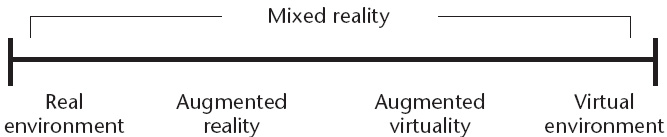
\includegraphics[width=9.5cm,height=2cm,angle=0]{/Users/enricopicchio/Desktop/TesiLaTex/IMG/priva.png}}
\caption{Reality-virtuality continuum, adapted from
Azuma et al. (2001).}
\end{figure}
%% Se si vuole più spazio usare il comando \vspace{0.35cm}

\newpage
%%%%%%%%%%%%%%%%%%%%%%%%%%%%%%%%%%%%%%%%%%%%%%%%%%%%%%%%
\section{Introduzione}
%%%%%%%%%%%%%%%%%%%%%%%%%%%%%%%%%%%%%%%%%%%%%%%%%%%%%%%%
\vspace{0.38cm}

\noindent % Comando per non fare partire il paragrafo con lo spazietto.
In representative democracies elected politicians take policy-relevant decisions on behalf of their constituency. Voters' decisions to support a particular candidate in an election for public office may have important policy consequences. Hence\footnote{A National sample of 797 adults from the 48 contiguous states was drawn. Respondents were questioned about their preferences and their perception about the position of a senator from their state on two policy issues (abortion and taxes) and on liberal-conservative dimension.}, individual voting behavior may contain information on citizens' political preferences. Many researchers in political science have focused on the characterization of the main determinants of voting. The general consensus is that\footnote{A National sample of 797 adults from the 48 contiguous states was drawn. Respondents were questioned about their preferences and their perception about the position of a senator from their state on two policy issues (abortion and taxes) and on liberal-conservative dimension.}, when voting, citizens are typically affected by three factors: party identification (that is, a voter's attachment to a particular party), policy preferences, and candidates' valence (that is, candidates' personal characteristics such as honesty, charisma, integrity, trustworthiness, or leadership). Voters will in general differ with respect to their policy and party preferences, but also to their level of political information. This generates a dilemma: democracy is actually based on people's choices, but people are poorly informed about fundamental political and economic questions. In 1989 in the USA, less than 50\% of the adult citizens knew which party had, at that time, a majority at the House (cf. Delli Carpini and Keeter, 1996). Indeed, one of the best documented features in contemporary politics is the ignorance of the American voter. Alvarez and Franklin (1994) conducted a survey in order to provide a direct measure of voters' lack of knowledge about elected officers' standpoints on public policy issues\footnote{A National sample of 797 adults from the 48 contiguous states was drawn. Respondents were questioned about their preferences and their perception about the position of a senator from their state on two policy issues (abortion and taxes) and on liberal-conservative dimension.}.Their study indicates that almost 50\% of the individuals were ''not very certain'' about politicians' position on taxes. This proportion exceeds 85\% when those that reported to be ''pretty certain'', yet not ''very certain'', are accounted for. These figures contrast sharply with the high level of certainty in self-placements, as only 10\% of respondents declared ''not very certain'' about their own option on this issue. This is interesting: people may have well defined opinions but they may fail to understand how these preferences can be mediated. \\
While American voters are often poorly informed, the same is true of their British counterparts. A recent survey by the British polling firm Ipsos MORI finds that most of the British public was ignorant or misinformed about basic facts relevant to the Brexit decision: voters had no idea what they were voting for. The polling firm get two important results:  an overestimation of the number of EU immigrants and the amount of child benefit, which was significant because fear of immigration was one of the main arguments put forward by the "leave" side, and an underestimation of investment by EU countries in Britain, which was relevant because one of the main arguments of the "remain" side was that Britain would have suffered serious economic harm from leaving the EU. Significantly, most of the examples of ignorance relevant to Brexit described in the Ipsos MORI poll seemed to help the "leave" side. According to their findings, if the British voted to leave the EU, ignorance might played a decisive role in the outcome. Indeed, this is what actually happened. \\
One of the biggest problems with modern democracy is that most of the public is usually ignorant of politics and government. Politics is complex: as voters are time constrained, and aware of the fact that they are unlikely to be pivotal in large election, they lack incentives to study all details and aspects of the political choices ahead. While most voters are therefore imperfectly informed about politics, the level of political information varies among people.\\
What are the consequences if some voters are better informed about politics, and thus better at picking the most suitable political party for themselves? In this model\footnote{A National sample of 797 adults from the 48 contiguous states was drawn. Respondents were questioned about their preferences and their perception about the position of a senator from their state on two policy issues (abortion and taxes) and on liberal-conservative dimension.}, we abandon the usual assumption of perfect information and assume instead that only a fraction of the voters is perfectly informed. In contrast with many theories arguing that the level of voters' information does not matter for the electoral outcome and policy implementation, we show that that incomplete information changes the equilibrium level of public good with respect to the full information case.\\
The remaining of this work is organized as follows. Section 2 discusses related literature. In Section 3 we describe the model; we derive the First Best and a full information benchmark in Section 4. We characterize the equilibrium of the electoral competition game and compare it with the benchmark in Section 5. Section 6 includes a brief digression on candidates' motivation. Section 7 concludes.
eeeeeeeeeeee

\begin{figure}[h!] % Le dimensioni massime per immagine sono  13.5cm(base)  e 10cm(altezza)
\centerline {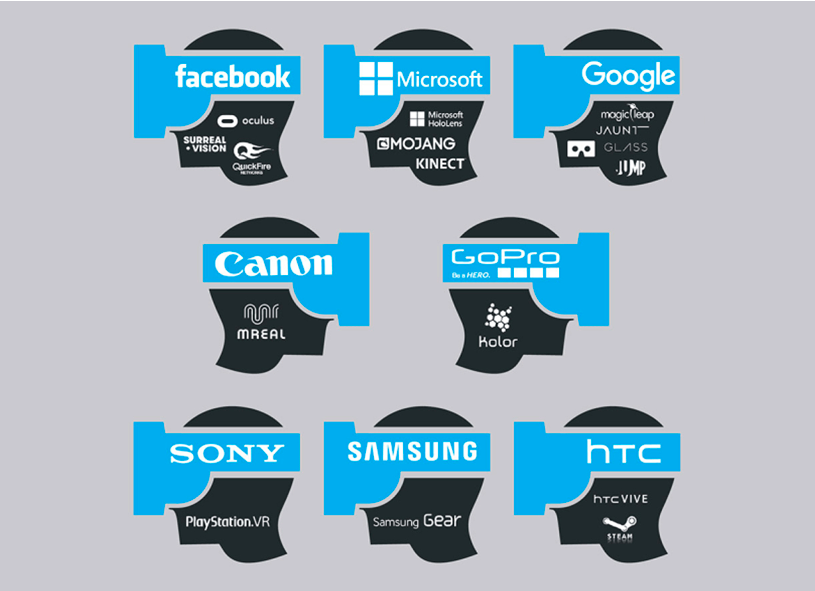
\includegraphics[width=13.8cm,height=10cm,angle=0]{/Users/enricopicchio/Desktop/TesiLaTex/IMG/provissima.pdf}}
\caption{Prova larghezza  testo}
\end{figure}

\newpage
\section{SPACE The future is all about communication}

\noindent
Sono appunti che mi sono segnato in biblioteca mentre  controllavo  la tesi di Mario.\\
\\
R. Kurzweil - "The primary political and philosophical issue of the next century will be the definition of who we are".\\
"Technology is an exponential process"\\
\\Consultare - https://www.kurzweilai.net/the-law-of-accelerating-returns\\
\\Consultare - http://startegy.it/kurzweil-la-tecnologia-e-un-processo-esponenziale/


\newpage
%%%%%%%%%%%%%%%%%%%%%%%%%%%%%%%%%%%%%%%%%%%%%%%%%%%%%%%%
\section{Introduzione}
%%%%%%%%%%%%%%%%%%%%%%%%%%%%%%%%%%%%%%%%%%%%%%%%%%%%%%%%

{\color{red}
\noindent % Comando per non fare partire il paragrafo con lo spazietto.
Testo.}

\newpage
%%%%%%%%%%%%%%%%%%%%%%%%%%%%%%%%%%%%%%%%%%%%%%%%%%%%%%%%
\section{Augmented Reality // Da Revisionare}
%%%%%%%%%%%%%%%%%%%%%%%%%%%%%%%%%%%%%%%%%%%%%%%%%%%%%%%%

\noindent % Comando per non fare partire il paragrafo con lo spazietto.
{\textbf{\textit{Augmented reality (AR)}} risulta come una variazione del cosiddetto {\textbf{\textit{virtual environment (VE)}}, comunemente noto come realtà virtuale,  consiste in un ambiente fittizio nel quale il soggetto umano ha la possibilità di interagire. La simulazione non risulterebbe quasi mai totale in quanto verrebbero coinvolti solo alcuni sensi.
Una prima differenza tangibile tra la {\textbf{virtual reality} e l’ambiente di realtà aumentata {\textbf{AR} è la possibilità di fruire dell’ambiente circostante, più precisamente, nel primo caso il soggetto che sta sfruttando la {\textbf{VR} non ha la possibilità di vedere ciò che lo circonda nel mondo reale, mentre l’{\textbf{AR} risulta come una tecnica di realtà virtuale, attraverso la quale si aggiungono informazioni alla scena reale. L’{\textbf{Augmented reality} amplifica la realtà arricchendola di dati, senza mai sostituirla completamente.
Oggetti virtuali e oggetti reali coesistono nello stesso momento e nel medesimo luogo.

{\color{red}
\noindent % Comando per non fare partire il paragrafo con lo spazietto.
Esempio del film Ready Player One di Spielberg per quanto riguarda la Virtual Reality e quindi un completa sostituzione del reale con il virtuale.\\}

\subsection{Campi di applicazione}

{\color{red}
\noindent % Comando per non fare partire il paragrafo con lo spazietto.
Lorem}












%%%%%%%%%%%%%%%%%%%%%%%%%%%%%%%%%%%%%%%%%%%%%%%%%%%%%%%%
%%                  Bibliografia                      %%
%%%%%%%%%%%%%%%%%%%%%%%%%%%%%%%%%%%%%%%%%%%%%%%%%%%%%%%%
\newpage
\selectlanguage{italian}
\begin{thebibliography}{50}

\addcontentsline{toc}{section}{\MakeUppercase{Bibliografia}}
\bibitem{einstein}
Alvarez R. M., Franklin C. H., 1994, ''Uncertainty and Political perceptions'', \textit {The journal of economics}: 671-688
\bibitem{einstein}
Austen-Smith D., Banks J., 1996, ''Information Aggregation, Rationality and the Condorcet Jury Theorem'', \textit {American Political Science Review} 90: 34-45
\bibitem{einstein}
Banks J. S., 1990, ''A model of electoral competition with incomplete information'',\textit {Journal of Economic Theory} 50: 309-25
\bibitem{einstein}
Baron, David P., 1994, ''Electoral competition with informed and uninformed voters'', \textit{American Political Science Review} 88: 33-47

\end{thebibliography}





\bibliographystyle{abbrv}
\bibliography{simple}


\end{document}
